\documentclass{ximera}

%\addPrintStyle{../..}


\begin{document}
	\author{Bart Lambregs, Vincent Gellens}
	\xmtitle{De positie}{}
    \xmsource\xmuitleg

\NewDocumentCommand{\maakachtvar}{m m m m m m m m}{

	\pgfmathsetmacro{\at}{#1}    \pgfmathsetmacro{\ax}{#2}
	\pgfmathsetmacro{\bt}{#3}    \pgfmathsetmacro{\bx}{#4}
	\pgfmathsetmacro{\ct}{#5}    \pgfmathsetmacro{\cx}{#6}
	\pgfmathsetmacro{\dt}{#7}    \pgfmathsetmacro{\dx}{#8}

	\pgfmathsetmacro{\tmin}{min(\at,\bt,\ct,\dt)}
	\pgfmathsetmacro{\tmax}{max(\at,\bt,\ct,\dt)}
	\pgfmathsetmacro{\xmin}{min(\ax,\bx,\cx,\dx)}
	\pgfmathsetmacro{\xmax}{max(\ax,\bx,\cx,\dx)}

	\pgfmathsetmacro{\deltat}{\tmax-\tmin}
	\pgfmathsetmacro{\deltax}{\xmax-\xmin}

	\pgfmathsetmacro{\xmargin}{0.08*\deltat}   
	\pgfmathsetmacro{\ymargin}{0.3*\deltax} 

	\pgfmathsetmacro{\xrangemin}{\tmin-\xmargin}
	\pgfmathsetmacro{\xrangemax}{\tmax+\xmargin}
	\pgfmathsetmacro{\yrangemin}{\xmin-\ymargin}
	\pgfmathsetmacro{\yrangemax}{\xmax+\ymargin}
}



\subsection*{Positie en plaatsfunctie}

Met behulp van een referentiestelsel kan elke plaats van een puntmassa in de ruimte worden beschreven met een \textbf{positie- of plaatsvector}, algemeen genoteerd door $\vec{r}$.
Afhankelijk van het aantal dimensies waarin de beweging beschreven wordt, heeft deze plaatsvector één, twee of drie componenten volgens de gekozen assen, doorgaans \(\vec{x}\), \(\vec{y}\) en \(\vec{z}\) genaamd.
De (scalaire) getalcomponenten van deze vectoren zijn de plaatscoördinaten \(x\),\(y\) en \(z\).




\begin{definition}
	De \textbf{positie} van een puntmassa \(A\) wordt vectorieel beschreven met de \textbf{plaatsvector \(\vec{r}\)}. % of scalair met behulp van de coördinaten \(x\) en \(y\). 
	Een plaatsvector \(\vec{r}\) kan ontbonden in de componenten volgens de assen.
	Op die manier krijgt de puntmassa \(A\) coördinaten \(co(A) = (x,y)\).  
	\[
	\vec{r} = \vec{x} + \vec{y} = \|\vec{x}\|\cdot\vec{e}_x + \|\vec{y}\|\cdot\vec{e}_y
	\]

\begin{image}[0.3\textwidth]
	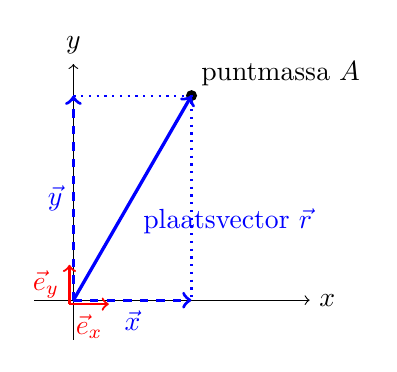
\begin{tikzpicture}
		\draw[->] (-0.5,0) -- (3,0) node[right] {$x$};
		\draw[->] (0,-0.5) -- (0,3) node[above] {$y$};
		\coordinate (O) at (0,0);

		\pgfmathsetmacro{\r}{3}       
		\pgfmathsetmacro{\ang}{60} 

		\coordinate (A) at (\ang :\r);
		\coordinate (X) at (\r*cos{\ang},0);
		\coordinate (Y) at (0,\r*sin{\ang});
	
		\fill (A) circle (2pt) node[above right] {puntmassa $A$};
	
		\draw[->, very thick, blue] (O) -- (A) node[midway, below right] {plaatsvector $\vec{r}$};
		\draw[->, very thick, dashed, blue] (O) -- (X) node[midway, below] {$\vec{x}$};
		\draw[->, very thick, dashed, blue] (O) -- (Y) node[midway, left] {$\vec{y}$};
		\draw[thick, dotted, blue] (Y) -- (A) -- (X);
	
		\draw[->, thick, red, transform canvas={shift={(-0.05,-0.05)}}] (O) -- (0.5,0) node[midway, below] {$\vec{e}_x$};
		\draw[->, thick, red, transform canvas={shift={(-0.05,-0.05)}}] (O) -- (0,0.5) node[midway, left] {$\vec{e}_y$};
	\end{tikzpicture}
\end{image}
\captionof{figure}{De plaatsvector \(\vec{r}\)}
\end{definition}


Als een puntmassa beweegt, verandert haar plaatsvector \(\vec{r}\).  
De beweging van een puntmassa wordt beschreven door een \textit{functie} die de \textbf{plaats} \(\vec{r}\) weergeeft in functie van de \textbf{tijd}. 
De \textbf{plaatsfunctie} \(\vec{r}\) = \(\vec{r}\)(t) geeft voor elk tijdstip \(t\) de positie \(\vec{r}\) waar de puntmassa zich bevindt. 
In het algemeen is een dergelijke vectorfunctie ingewikkeld om te hanteren, daarom wordt er gewerkt met de tijdsafhankelijke getalcomponenten \(x(t)\),\(y(t)\) en \(z(t)\).
Elke coördinaatfunctie geeft voor elk moment \(t\) de coördinaat van de puntmassa volgens een welbepaalde-as. 
Al deze componentfuncties samen beschrijven de volledige beweging van de puntmassa. 


Bij ééndimensionale bewegingen is er slechts één coördinaatas nodig om de beweging te beschrijven. 
Op die as wordt de positie als scalar afgelezen, de waarde ervan is afhankelijk van de tijd \(t\). 
\footnote{In fysica gebruiken we wiskunde als `taal' om de wetmatigheden van de natuur uit te drukken. 
Wiskundige variabelen en objecten zoals functies krijgen nu een fysische betekenis. 
$x(t)$ is dus niets anders dan een functie $f(x)$ of $y(x)$ zoals je die in wiskunde kent. 
Alleen nemen wij nu niet voor de onafhankelijke variabele het symbool $x$, maar het symbool $t$. 
En voor het symbool $f$ gebruiken wij nu het symbool $x$ omdat die de beeldwaarden zijn van de functie \(f\), \(x\) is afhankelijk van \(t\).}


De positie op een welbepaald tijdstip $t_1$ wordt genoteerd als 
\footnote{Natuurlijk kan de index 1 ook vervangen worden door andere indices. Voorbeelden zijn $x_0=x(t_0)$ en $x_2=x(t_2)$.} 
\begin{eqnarray*}
x_1=x(t_1)
\end{eqnarray*}

In onderstaande figuur zie je de rechtlijnige tocht van een zeilship. 
Op verschillende tijdstippen $t_0,t_1, t_2,\ldots$ wordt weergegeven waar het schip zich bevindt. 


\maakachtvar{0}{30}{5}{40}{15}{10}{35}{-10}

\begin{image}[0.8\textwidth]
  \begin{tikzpicture}
  \begin{axis}[
	  axis x line=bottom,
	  axis y line=none,   
	  axis line style={->},
	  xmin= \yrangemin, xmax=\yrangemax,
	  ymin=-1, ymax=3,  %plek voor schepen en tijdlabels 
	  xlabel={Positie--as (in meter)},
	  xtick distance=5,
	  xticklabel={\tiny\SI[round-precision=0, round-mode=places]{\tick}{m}},
	  width=14cm, height=4cm,
  ]

  \node[opacity=0.3,scale=1,xscale=-1]  (ship1) at (axis cs:\ax,0.5)  {
\includegraphics[width=1cm]{schip_icoon}};
  \node[draw, rectangle, inner sep=1pt] (t1) at (axis cs:\ax,2.2) {\small $t_0=\SI{\at}{\second}$};

  \node[opacity=0.6,scale=1,xscale=0.7] (ship2) at (axis cs:\bx,0.5)  {
\includegraphics[width=1cm]{schip_icoon}};
  \node[draw, rectangle, inner sep=1pt] (t2) at (axis cs:\bx,2.2) {\small $t_1=\SI{\bt}{\second}$};

  \node[opacity=0.9]                     (ship3) at (axis cs:\cx,0.5) {
\includegraphics[width=1cm]{schip_icoon}};
  \node[draw, rectangle, inner sep=1pt] (t3) at (axis cs:\cx,2.2) {\small $t_2=\SI{\ct}{\second}$};

  \node[]                                (ship4) at (axis cs:\dx,0.5) {
\includegraphics[width=1cm]{schip_icoon}};
  \node[draw, rectangle, inner sep=1pt] (t4) at (axis cs:\dx,2.2) {\small $t_3=\SI{\dt}{\second}$};
  
  \end{axis}
  \end{tikzpicture}
\end{image}
\captionof{figure}{De positie van de zeilboot voor elke tijd \(t\)}


% @Bart; Vincent stelt voor 'tijd is dimensie' en voetnoot Einstein te laten vallen (draagt niet bij tot begrip van deze materie, kan verwarrend zijn, niet relevant om te vermelden)
In de natuurkunde is \textbf{tijd een dimensie}.\footnote{Einstein gaf een beschrijving voor de zwaartekracht in de \textit{4-dimensionale ruimte-tijd}.}
In bovenstaande figuur wordt boven elke zeilboot aangegeven op welk tijdstip de boot daar werd waargenomen. 
Zo bevindt de boot zich op \(t_1 = \SI{5}{\second}\) op de positie \SI{40}{\meter}, dus \(x_1 = \SI{40}{\meter}\). 
De startpositie van de zeilboot \(x_0\) is gelijk aan \(\SI{30}{\meter}\), want voor \(t_0 = \SI{0}{\second}\) geldt \(x(0) = \SI{30}{\meter}\).
In plaats van de tijd boven elke zeilboot te noteren, is het ook mogelijk om de tocht op een tijd-as uit te zetten. 


\begin{image}[0.5\textwidth]
	\begin{tikzpicture}
		\begin{axis}[
			axis x line=bottom,
			axis y line=left,
			axis line style={->},
			xlabel={tijd (in seconden)},
			ylabel={positie (in meter)},
			xmin= \xrangemin, xmax=\xrangemax,
			ymin= \yrangemin, ymax=\yrangemax,
			xtick distance=5,
			ytick distance=10,
			xticklabel={\SI[round-precision=0, round-mode=places]{\tick}{s}},
			yticklabel={\SI[round-precision=0, round-mode=places]{\tick}{m}},
			grid=both,
			width=15cm, height=10cm,
		]
		
		\node[] at (axis cs:\at,\ax) {
\includegraphics[width=1cm]{schip_icoon}};
		\node[draw, rectangle, inner sep=1pt] at (axis cs:\at,\ax+10) {\small $t_0=\SI{\at}{\second}$};
	
		\node[] at (axis cs:\bt,\bx) {
\includegraphics[width=1cm]{schip_icoon}};
		\node[draw, rectangle, inner sep=1pt] at (axis cs:\bt,\bx+10) {\small $t_1=\SI{\bt}{\second}$};
	
		\node[] at (axis cs:\ct,\cx) {
\includegraphics[width=1cm]{schip_icoon}};
		\node[draw, rectangle, inner sep=1pt] at (axis cs:\ct,\cx+10) {\small $t_2=\SI{\ct}{\second}$};
	
		\node[] at (axis cs:\dt,\dx) {
\includegraphics[width=1cm]{schip_icoon}};
		\node[draw, rectangle, inner sep=1pt] at (axis cs:\dt,\dx+10) {\small $t_3=\SI{\dt}{\second}$};
	
		\end{axis}
		\end{tikzpicture}
	\end{image}
	\captionof{figure}{De positie van de zeilboot met een tijd-as}
	
	
	

% @Bart vincent stelt voor deze paragraaf te laten vallen (helft van de lln gaat flippen; leuk voor enkele slimme gasten; voor meeste leerlingen is dit ontmoedigend)
Er zit \textbf{geen} extra informatie in bovenstaande figuur! 
We hebben enkel de tijdsdimensie uitgezet op een horizontale-as en de positie op de verticale-as. 
Als je nu ijverig natuurkunde aan het studeren bent, kan je 'de positie' van dit blad papier onderzoeken. 
Dit blad ligt stil op je bureau en je probeert te begrijpen wat er uitgelegd wordt. 
Dan verandert de positie volgens de positie-as natuurlijk niet, maar het blad beweegt zich wel voort op de tijd-as. \footnote{Want terwijl je dit aan het lezen bent staat de tijd natuurlijk niet stil...\footnotemark}
\footnotetext{Je blad beweegt zich -eerder saai- constant voort op de tijdsdimensie. Het is echter mogelijk -in de relativiteitstheorie- om ook op meer interessantere manieren op de tijd-as te bewegen.\footnotemark}
\footnotetext{Aangezien je enkel constant op de tijd-as kan voortbewegen, en dus niet terug kan, lijkt het aangewezen om je tijd goed te benutten. Bijvoorbeeld door wat natuurkunde te leren.}



De positie van de zeilboot is enkel weergegeven voor een aantal specifieke momenten \(t_0, t_1, t_2, t_3 \text{ en } t_4\). 
De boot heeft natuurlijk ook op \textit{elk moment hiertussen} een positie \ldots


\begin{image}[0.8\textwidth]
	\begin{tikzpicture}
		\begin{axis}[
			axis x line=bottom,
			axis y line=left,
			axis line style={->},
			xlabel={tijd (in seconden)},
			ylabel={positie (in meter)},
			xmin= \xrangemin, xmax=\xrangemax,
			ymin= \yrangemin, ymax=\yrangemax,
			xtick distance=5,
			ytick distance=10,
			xticklabel={\SI[round-precision=0, round-mode=places]{\tick}{s}},
			yticklabel={\SI[round-precision=0, round-mode=places]{\tick}{m}},
			grid=both,
			width=15cm, height=10cm,
		]
		
		\addplot[blue, thick, smooth, tension=0.5] coordinates{
			(\at,\ax)
			(\bt,\bx)
			(\ct,\cx)
			(\dt,\dx)
		};
		
		\node[] at (axis cs:\at,\ax) {
\includegraphics[width=1cm]{schip_icoon}};
		\node[draw, rectangle, inner sep=1pt] at (axis cs:\at,\ax+10) {\small $t_0=\SI{\at}{\second}$};
	
		\node[] at (axis cs:\bt,\bx) {
\includegraphics[width=1cm]{schip_icoon}};
		\node[draw, rectangle, inner sep=1pt] at (axis cs:\bt,\bx+10) {\small $t_1=\SI{\bt}{\second}$};
	
		\node[] at (axis cs:\ct,\cx) {
\includegraphics[width=1cm]{schip_icoon}};
		\node[draw, rectangle, inner sep=1pt] at (axis cs:\ct,\cx+10) {\small $t_2=\SI{\ct}{\second}$};
	
		\node[] at (axis cs:\dt,\dx) {
\includegraphics[width=1cm]{schip_icoon}};
		\node[draw, rectangle, inner sep=1pt] at (axis cs:\dt,\dx+10) {\small $t_3=\SI{\dt}{\second}$};
		\end{axis}
	\end{tikzpicture}
	
	\begin{tikzpicture}
			\begin{axis}[
				axis x line=bottom,
				axis y line=left,
				axis line style={->},
				xlabel={tijd (in seconden)},
				ylabel={positie (in meter)},
				xmin= \xrangemin, xmax=\xrangemax,
				ymin= \yrangemin, ymax=\yrangemax,
				xtick distance=5,
				ytick distance=10,
				xticklabel={\SI[round-precision=0, round-mode=places]{\tick}{s}},
				yticklabel={\SI[round-precision=0, round-mode=places]{\tick}{m}},
				grid=both,
				width=15cm, height=10cm,
			]
			
			\addplot[blue, thick, smooth, tension=0.5] coordinates{
				(\at,\ax)
				(\bt,\bx)
				(\ct,\cx)
				(\dt,\dx)
			};
			
			\end{axis}
			\end{tikzpicture}
	\end{image}
	\captionof{figure}{De plaatsfunctie van de zeilboot voor elke \(t \in [0, 35]\)}

\begin{definition} 
	De \textbf{plaatsfunctie} \(\vec{x}(t)\) geeft voor elke moment \(t\) de positievector \(\vec{x}\). \\
	In één dimensie heeft \(\vec{x}\) maar één getalcomponent, namelijk \(x\) die ook tijdsafhankelijk is. 
	\(x(t)\) geeft de plaatsfunctie die je kan uitzetten in een grafiek met verticale \(x\)-as en horizontale \(t\)-as. 
	De positie op een welbepaald tijdstip \(t_a\) wordt genoteerd als 
	\[
	x_a = x(t_a)
	\]

\begin{image}[0.3\textwidth]
	\begin{tikzpicture}
		\begin{axis}[
			axis lines=middle,
			xlabel={tijd \(t\)}, ylabel={positie \(x\)},
			grid=both,
			width=10cm, height=6cm,
			xmin=0, xmax=6, ymin=0, ymax=6,
			xtick=\empty,
			ytick=\empty,
			clip=false,
		]
		\addplot[
			only marks,
			mark=*,
			mark size=2pt,
			color=red
		] coordinates {
			(3,2) (5,5)
		};
	
		\addplot[
			smooth,
			thick,
			color=blue
		] coordinates {
			(0,1) (1,3) (3,2) (5,5) (6,5.5)
		};

		\draw[dashed] (axis cs:3,2) -- (axis cs:3,0) node[below]{$t_a$};
		\draw[dashed] (axis cs:3,2) -- (axis cs:0,2) node[left]{$x_a$};
		\draw[dashed] (axis cs:5,5) -- (axis cs:5,0) node[below]{$t_b$};
		\draw[dashed] (axis cs:5,5) -- (axis cs:0,5) node[left]{$x_b$};

		\end{axis}
	\end{tikzpicture}
\end{image}
\captionof{figure}{De grafiek van een plaatsfunctie \(x(t)\)}

\end{definition}


\begin{remark} 
	In één dimensie is het onderscheid tussen een 'vector' $\vec{x}$ en een 'getal' $x$ erg klein: beide kunnen volledig de positie beschrijven. 
	In twee of drie dimensies kan je de positie wel beschrijven met één vector $\vec{x}$, maar heb je twee of drie getallen $x,y$ of $x,y,z$ nodig.
\end{remark}
	
De \textbf{verplaatsing} tussen $t_1$ en $t_2$ is het verschil in positie tussen de twee tijdstippen $t_1$ en $t_2$, genoteerd met een $\Delta$\(\vec{r}\) (Delta, een Griekse hoofdletter D  van het Engelse 'displacement' of het Franse 'déplacement').

\begin{definition}
De \textbf{verplaatsing} \(\Delta \vec{r}\) is het verschil tussen twee posities:
\[
\Delta \vec{r}_{21} = \vec{r}_2 - \vec{r}_1
\]

\tikzset{>={latex[scale=1.2]}}
\begin{image}[0.3\textwidth]
	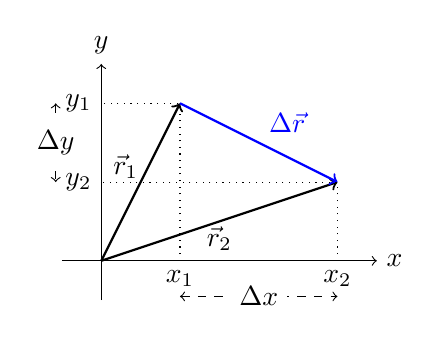
\begin{tikzpicture}
		
		\draw[->] (-0.5,0) -- (3.5,0) node[right] {$x$};
		\draw[->] (0,-0.5) -- (0,2.5) node[above] {$y$};
		
		\coordinate (A) at (1,2);
		\coordinate (AX) at (1,0);
		\coordinate (AY) at (0,2);

		\coordinate (B) at (3,1);
		\coordinate (BX) at (3,0);
		\coordinate (BY) at (0,1);
		
		\draw[->, thick] (0,0) -- (A) node[pos= 0.6, left] {$\vec{r}_1$};
		\draw[->, thick] (0,0) -- (B) node[midway, below, yshift=2pt] {$\vec{r}_2$};
		\draw[->, thick, blue] (A) -- (B) node[midway, above right] { $\Delta \vec{r}$};

		\node[below] (ax) at (AX) {\(x_1\)};
		\node[left] (ay) at (AY) {\(y_1\)};
		\node[below] (bx) at (BX) {\(x_2\)};
		\node[left] (by) at (BY) {\(y_2\)};
		
		\draw[dotted, thin] (AX) -- (A) -- (AY);
		\draw[dotted, thin] (BX) -- (B) -- (BY);

		\draw[<->, dashed] (ax.south) -- (bx.south) node[midway, fill=white]{\(\Delta x\)};
		\draw[<->, dashed] (ay.west) -- (by.west) node[midway, fill=white]{\(\Delta y\)};

	\end{tikzpicture}
\end{image}


Zoals aangegeven in de figuur kan ook de verplaatsingsvector \(\Delta\vec{r}\) ontbonden worden. 

\begin{align*}
\Delta\vec{r}_{21} &= \vec{r}_2 - \vec{r}_1 \\ 
					&= (x_2\cdot\vec{e}_x + y_2\cdot\vec{e}_y) - (x_1\cdot\vec{e}_x + y_1\cdot\vec{e}_y) \\
					&= (x_2-x_1)\cdot\vec{e}_x + (y_2-y_1)\cdot\vec{e}_y \\
					&= \Delta x \cdot\vec{e}_x + \Delta y \cdot\vec{e}_y
\end{align*}


\end{definition}

Voor ééndimensionale bewegingen is de verplaatsing eenvoudig scalair te berekenen met: $\Delta x$ = $x_{eind}-x_{begin}$.
De verplaatsing van de zeilboot tussen de tijdstippen $t_0$ en $t_1$ is gelijk aan \( \Delta x = x_1-x_0 = \SI{40}{\meter} - \SI{30}{\meter} = \SI{10}{\meter}\).  
Tussen $t_2$ en $t_3$ is de verplaatsing gelijk aan \(\Delta x = x_3 - x_2=\SI{-10}{\meter} - \SI{10}{\meter} = \SI{-20}{\meter}\). 
Deze laatste verplaatsing is negatief, wat aangeeft dat de zeilboot netto naar achteren is bewogen -- tegengesteld aan de zin van de gekozen as.
Op de plaatsfunctie kan de verplaatsing eenvoudig afgelezen worden: 

\begin{image}
	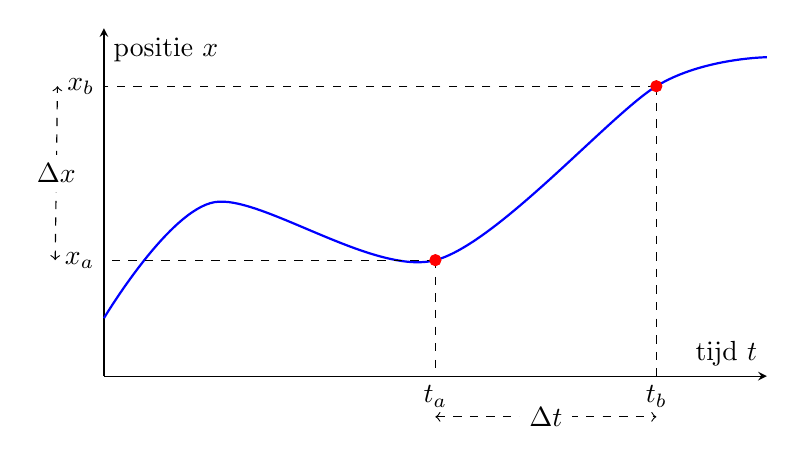
\begin{tikzpicture}
		\begin{axis}[
			axis lines=middle,
			xlabel={tijd \(t\)}, ylabel={positie \(x\)},
			grid=both,
			width=10cm, height=6cm,
			xmin=0, xmax=6, ymin=0, ymax=6,
			xtick=\empty,
			ytick=\empty,
			clip=false,
		]
		\addplot[
			only marks,
			mark=*,
			mark size=2pt,
			color=red
		] coordinates {
			(3,2) (5,5)
		};
	
		\addplot[
			smooth,
			thick,
			color=blue
		] coordinates {
			(0,1) (1,3) (3,2) (5,5) (6,5.5)
		};

		\draw[dashed] (axis cs:3,2) -- (axis cs:3,0) node[below] (tijda) {$t_a$};
		\draw[dashed] (axis cs:3,2) -- (axis cs:0,2) node[left] (posa) {$x_a$};
		\draw[dashed] (axis cs:5,5) -- (axis cs:5,0) node[below] (tijdb) {$t_b$};
		\draw[dashed] (axis cs:5,5) -- (axis cs:0,5) node[left] (posb){$x_b$};

		\draw[<->, dashed] (tijda.south) -- (tijdb.south) node[midway, fill=white]{\(\Delta t\)};
		\draw[<->, dashed] (posa.west) -- (posb.west) node[midway, fill=white]{\(\Delta x\)};

		\end{axis}
	\end{tikzpicture}
\end{image}
\captionof{figure}{De verplaatsing op de plaatsfunctie}

\begin{quickquestion*}{}{}
Bereken de verplaatsing \(\Delta x = x_4 - x_1\) van de zeilboot en duid deze verplaatsing aan op de grafiek.  
\end{quickquestion*}


Wanneer een voorwerp beweegt, doorloopt het meerdere posities. 
De verbindingslijn van al deze gepasseerde posities, noemt men de \textbf{baan} van de beweging. 
Een ééndimensionale beweging heeft een rechte baan. 
Een tweedimensionale is doorgaans krom en kan meerdere vormen hebben (willekeurig, cirkelvormig, paraboolvormig, ellipsvormig,\ldots). 
Soms is men geïnteresseerd in een \textbf{baanvergelijking} waarin men de afhankelijkheid tussen x en y wiskundig neerschrijft.
Indien de functies \(x(t)\) en \(y(t)\) gekend zijn, kan soms een (expliciete) baanvergelijking bekomen worden door één voorschrift uit te werken naar \(t\) en dit vervolgens te substitueren in de andere vergelijking.


% Hier zijn betere voorbeelden --> je wilt de baan wss ook kunnen plotten etc (bv cos en sin --> de baan is een cirkel; dan bij ECR hiernaar verwijzen...?)(miss voor volgend jaar)
\begin{example}
De positie van puntmassa \(A\) in het \(xy\)-vlak wordt gegeven door 

\[
\left\{
\begin{array}{l}
	x = t^7 \\ 
	y = -t^2 - 3t
\end{array}
\right.
\]


Een rechtstreekse berekening levert \( x = t^7 \Rightarrow t = \sqrt[7]{x} \). 
Dit substitueren in het voorschrift \(y(t)\) geeft de baanvergelijking \(y(x)\): 

\[
y = -t^2 - 3t \Rightarrow y(x) = -(\sqrt[7]{x})^2 - 3\sqrt[7]{x}
\]


\end{example}


Let op: de \textit{verplaatsing} is niet hetzelfde als de \emph{afgelegde weg} tussen de twee bijbehorende tijdstippen. 
Als je een rondje hebt gelopen op de atletiekpiste en terug aan start staat is je (netto) verplaatsing nul, maar jet hebt wel degelijk afstand afgelegd.
De verplaatsing geeft enkel het verschil (in vogelvlucht) tussen begin- en eindpunt, terwijl de afgelegde weg \(s\) gaat over de afstand die het bewegende voorwerp over zijn baan aflegt. 

\begin{image}[0.5\textwidth]

\begin{tikzpicture}[scale=1.1]
	\node[left] (A) at (0,0) {A};
	\node[right] (B) at (6,2) {B};
  
	\draw[thick,->] (A) -- (B) node[midway, above]{\(\Delta \vec{x}\)};
  
	\draw[dashed] 
	  (A) .. controls (2,2) and (4,3) .. (B) 
	  node[midway,above left] {baan \(1\)};
  
	\draw[dashed] 
	  (A) .. controls (2,-0.5) and (3,-1.5) .. (3,-1.8)
		  .. controls (3,-2.2) and (2.5,-2.2) .. (3,-1.5)
		  .. controls (3.5,-1) and (5,0) .. (B)
	  node[midway,right] {baan \(2\)};
  
  \end{tikzpicture}
\end{image}
\captionof{figure}{Verplaatsing en afgelegde weg}

% Samengevat voor ééndimensionale bewegingen:

% OMGEZET NAAR TABULARS
% \begin{image}
% 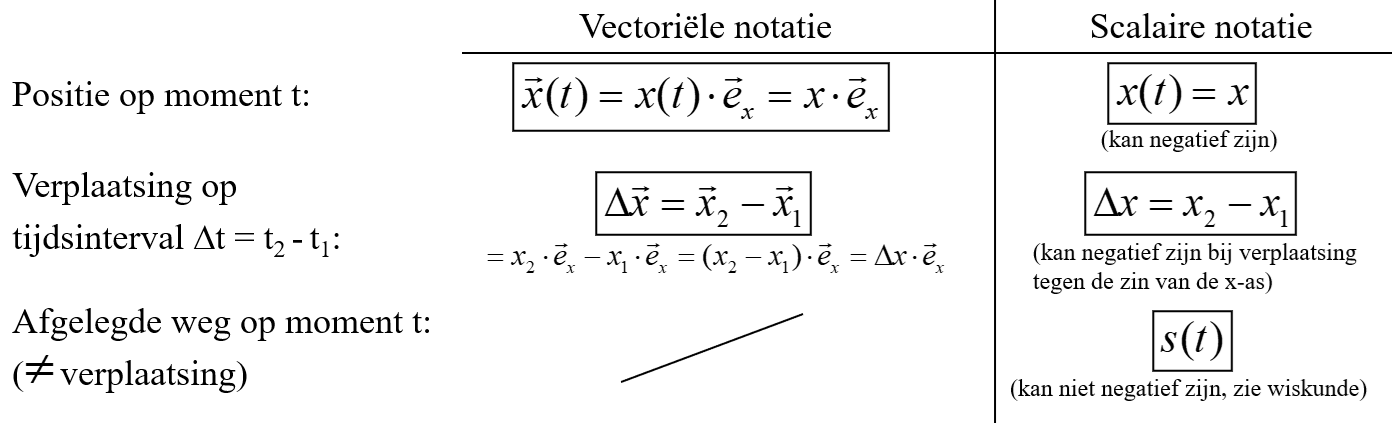
\includegraphics[width=0.8\textwidth]{positieverplaatsing1D}

% \end{image}



% SCALAIR EN VECTORIEEL NOG OMDRAAIEN
% \fbox{
% \begin{tabular}{p{5cm} >{\centering\arraybackslash}p{5cm} >{\centering\arraybackslash\arraybackslash}p{5cm}}
% 																		& Vectoriële notatie                                            & Scalaire notatie        \\ [4pt]
% 	% \cline{2-3}\noalign{\vskip 8pt}
% 	Positie op moment \(t\):                                            & \fbox{$\vec{x}_t = x(t)\cdot\vec{e}_x = x\cdot\vec{e}_x $ }   & \fbox{$x(t) = x$}  \newline \tiny{(kan negatief zijn)}             \\ [15pt]
% 	Verplaatsing op het \newline tijdsinterval $\Delta t = t_2 - t_1 $: & \fbox{$\Delta\vec{x} = \vec{x}_2 - \vec{x}_1$} \newline \tiny{$\Delta x \cdot \vec{e}_x = (x_2-x_1)\cdot \vec{e}_x = x_2\cdot\vec{e}_x - x_1\cdot\vec{e}_x$ } & \fbox{$\Delta x = x_2 - x_1 $} \newline \tiny{(kan negatief zijn bij een verplaatsing tegen de zin van de \(x\)-as.)}\\ [20pt]
% 	Afgelegde weg op moment t:                                          &  $\diagup$                                                    & $s(t)$ \newline \tiny{kan negatief zijn; zie wiskunde}
% \end{tabular}
% }
	



% Voor tweedimensionale bewegingen worden de begrippen positie, verplaatsing en afgelegde weg complexer.

% \begin{image}
% 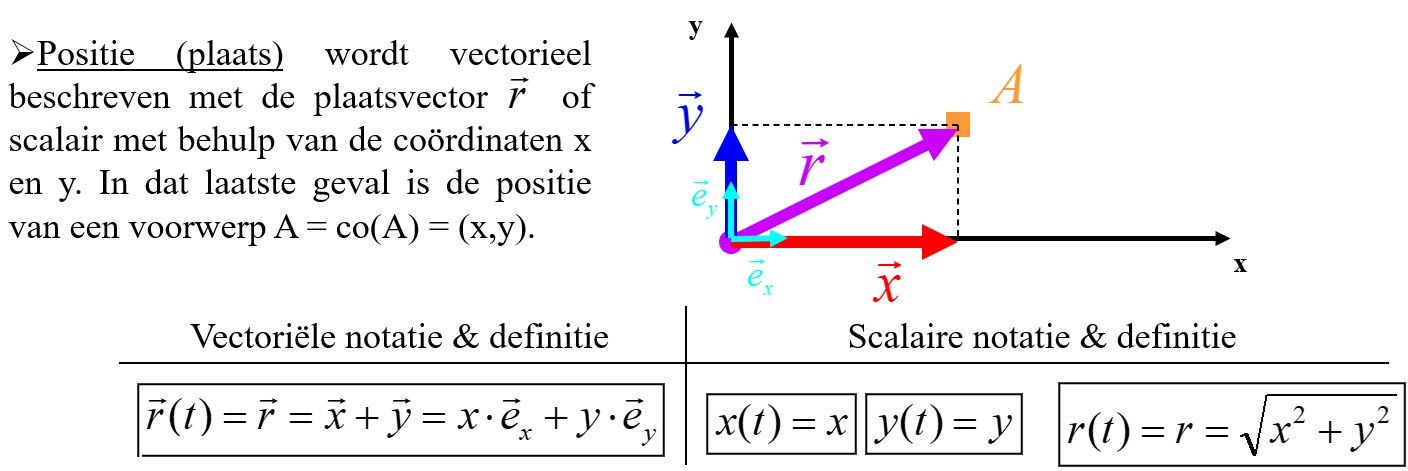
\includegraphics[width=0.8\textwidth]{positie2D}

% \end{image}



% \begin{image}
% 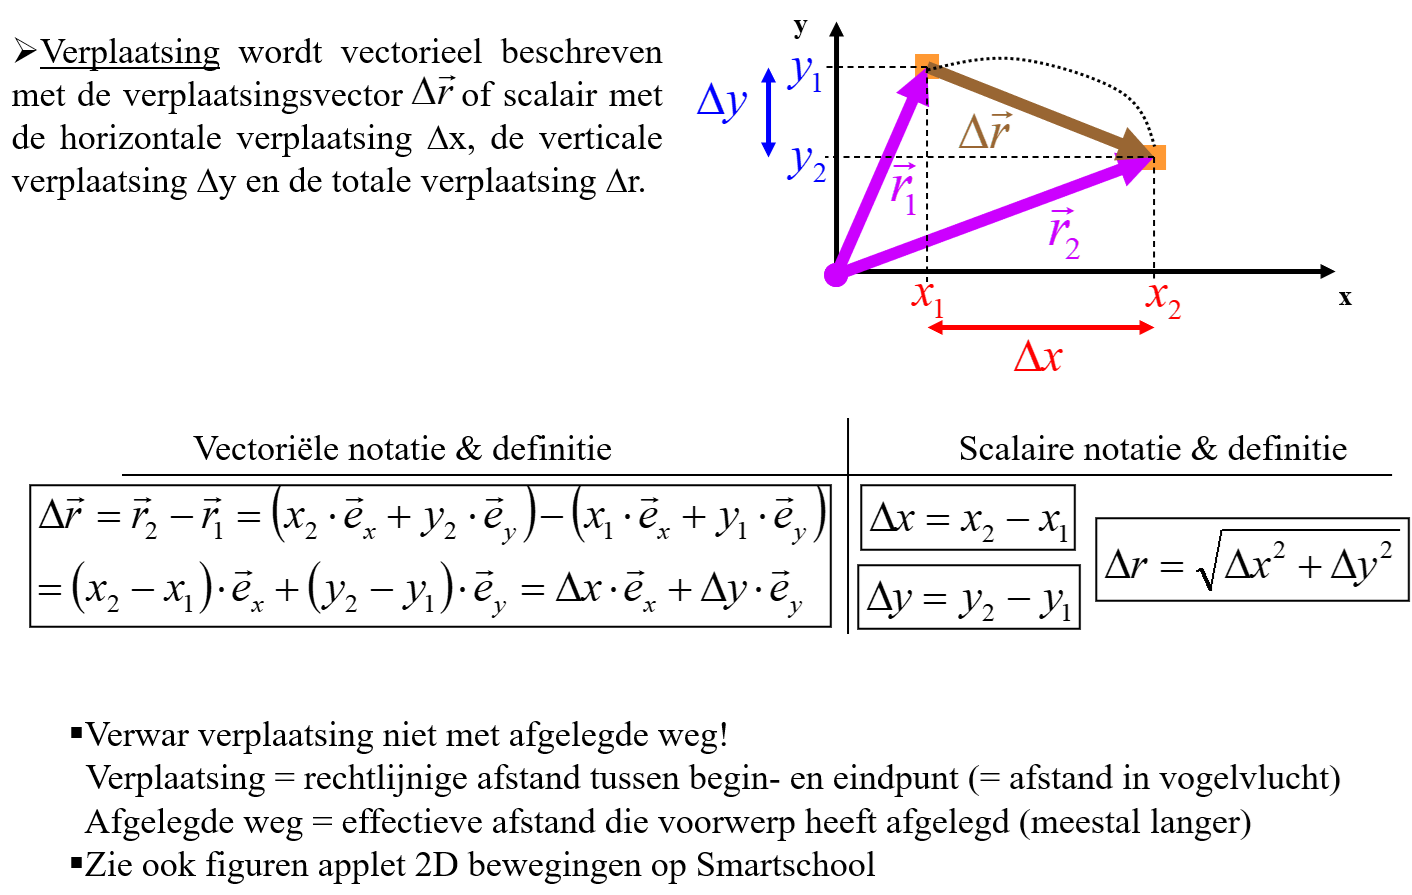
\includegraphics[width=0.8\textwidth]{verplaatsing2D}

% \end{image}


% \begin{image}
% 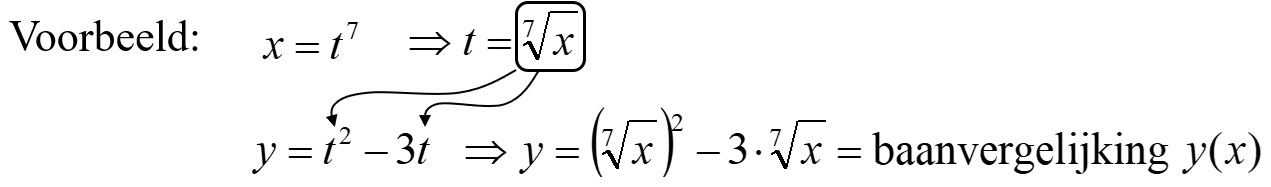
\includegraphics[width=0.8\textwidth]{vbBaanvergelijking}

% \end{image}
	
\end{document}






% DIT WAS EEN TEST OM DIE SINUS UIT HET HANDBOEK NA TE MAKEN 
% \begin{image}
% 	\begin{tikzpicture}
% 	\begin{axis}[
% 		axis x line=bottom,
% 		axis y line=left,
% 		xlabel={$x$}, ylabel={$y$},
% 		xmin=0, xmax=50,              % x-axis 0 to 50
% 		ymin=-45, ymax=60,            % y-axis -60 to 60
% 		xtick={0,10,...,50},          % x ticks every 10
% 		ytick={-60,-50,...,60},       % y ticks every 10
% 		grid=both,
% 		width=12cm, height=6cm,
% 		samples=200,
% 		domain=0:50,
% 		axis line style={->},         % arrows at ends
% 		% scale y visually double the x
% 		x=0.2cm,                      % compress x
% 		y=0.1cm,                      % stretch y
% 		enlarge y limits=0.05,
% 	]
% 		% scaled sine function to fit -60..60
% 		\addplot[blue, thick] {60*sin(deg((pi/50)*x + pi/4))};
% 	\end{axis}
% 	\end{tikzpicture}
% \end{image}
